\documentclass[a4paper,12pt]{article}
\usepackage{fullpage}
\usepackage{amsmath}
\usepackage{graphicx}
\usepackage{subfig}
\usepackage{bm}
\usepackage{amssymb}
\usepackage{fixltx2e}
\usepackage[nodisplayskipstretch]{setspace}
\usepackage{etoolbox}

\usepackage[margin=0.75in]{geometry}

\BeforeBeginEnvironment{equation}{\begin{singlespace}}
\AfterEndEnvironment{equation}{\end{singlespace}\noindent\ignorespaces}
%\BeforeBeginEnvironment{align}{\begin{singlespace}}
%\AfterEndEnvironment{align}{\end{singlespace}\noindent\ignorespaces}
%\BeforeBeginEnvironment{eqnarray}{\begin{singlespace}}
%\AfterEndEnvironment{eqnarray}{\end{singlespace}\noindent\ignorespaces}

\usepackage[compact]{titlesec}
\titlespacing{\section}{0pt}{*0}{*0}
\titlespacing{\subsection}{0pt}{*0}{*0}
\titlespacing{\subsubsection}{0pt}{*0}{*0}

\setlength{\abovedisplayskip}{0pt}
\setlength{\belowdisplayskip}{0pt}
\setlength{\abovedisplayshortskip}{0pt}
\setlength{\belowdisplayshortskip}{0pt}

\allowdisplaybreaks

\renewcommand{\vec}[1]{\boldsymbol{\mathbf{#1}}}

\begin{document}

%\begin{flushright}
%Dillon Wong \\
%\end{flushright}

\begin{center}
\mbox{} \\
{ \large Dirac Cones of the Kagome Lattice}
\end{center}

\doublespacing

The Kagome lattice is famous for its flat band.  Although one could explicitly calculate the tight-binding band structure of the Kagome lattice, a slick, well-known argument for the existence of the flat bands is to put +1 and -1 phases on alternating atoms of a hexagonal plaquette.  This distribution of phases leads to destructive interference outside the plaquette, producing a spatially localized energy eigenstate.  Then, one could take superpositions of this state translated onto all other plaquettes to build Bloch wavefunctions, all with the same energy.

A more general proof involves the idea of line graphs.  Suppose you had an undirected graph $G$ (called the root graph). The line graph $L(G)$ is the graph constructed by placing a vertex on each edge of $G$.  Then, pairs of vertices $u$ and $w$ in $L(G)$ are connected if and only if the corresponding edges for $u$ and $w$ in $G$ share a common vertex in $G$.  It turns out that under certain conditions (consult the references for more details), if vertices represent atomic sites and edges represent hopping terms in the Hamiltonian, the band structure of the graph $G$ is the same as the band structure of $L(G)$ except with $n(d-2)/2$ flat bands.  Here, $n$ is the number of vertices per unit cell, and $d$ is the coordination number for the atoms.

The punchline here is that the Kagome lattice is the line graph of the honeycomb (graphene) lattice.  Hence, there are Dirac cones\footnote{Which was required by symmetry anyway.} and a flat band in the band structure.  While the proof of the relationship between the band structures of $G$ and $L(G)$ is really cool, it definitely isn't obvious.  Here, I present an alternate proof that the dispersive band of the Kagome lattice is the same as that of the honeycomb lattice.

Suppose we have an eigenstate of the honeycomb Hamiltonian:
\begin{equation}
\label{eq:schro_graphene}
H_G | \Psi_G \rangle = \epsilon_G | \Psi_G \rangle
\end{equation}
where
\begin{equation}
H_G = -t \sum_{\langle ij \rangle} c_i^\dagger c_j +  c_j^\dagger c_i
\end{equation}
The sum is taken over nearest-neighbor atoms on the honeycomb lattice.  The Hamiltonian for the Kagome lattice $H_K$ has the same form except the arrangement of atoms and nearest-neighbors bonds are different.

Now I will index the localized orbitals on the root graph $G$ (i.e. the honeycomb lattice) by numerals $| 1 \rangle$, $| 2 \rangle$, etc..., while the orbitals on the line graphene $L(G)$ (i.e. the Kagome lattice) are indexed by letters $| A \rangle$, $| B \rangle$, etc...  Please take a look at the figure below.

\begin{figure}[h!]
\centering
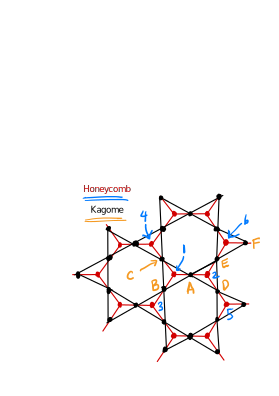
\includegraphics[width=70mm,keepaspectratio=true]{line-graph.png}
\end{figure}

Multiplying Eq. \ref{eq:schro_graphene}. by $\langle 1 |$ and $\langle 2 |$ gives
\begin{align}
-t (\Gamma_2 + \Gamma_3 + \Gamma_4) = \epsilon_G \Gamma_1 \\
-t (\Gamma_1 + \Gamma_5 + \Gamma_6) = \epsilon_G \Gamma_2
\end{align}
where $\Gamma_i = \langle i | \Psi_G \rangle$.

Now let's construct an ansatz state on the Kagome lattice:
\begin{equation}
|\Psi_K \rangle = \sum_{j \in L(G)} \sum_{i} \Gamma_i | j \rangle
\end{equation}
where for each orbital $j$ on the Kagome lattice, $i$ runs through all vertices on the root graph $G$ that are endpoints of the edge in $G$ corresponding to $j$.  In other words, if vertex $j \in L(G)$ corresponds to an edge $(u, w) \in G$, then $\sum_i \Gamma_i | j \rangle = (\Gamma_u + \Gamma_w) | j \rangle$.  With the notation that $\Lambda_j = \langle j | \Psi_K \rangle$, his gives us the following relations:
\begin{align}
\Lambda_A = \Gamma_1 + \Gamma_2 \\
\Lambda_B = \Gamma_1 + \Gamma_3 \\
\Lambda_C = \Gamma_1 + \Gamma_4 \\
\Lambda_D = \Gamma_2 + \Gamma_5 \\
\Lambda_E = \Gamma_2 + \Gamma_6
\end{align}

Now let's calculate
\begin{align}
\langle A | H_K | \Psi_K \rangle &= -t (\Lambda_B + \Lambda_C + \Lambda_D + \Lambda_E) \\
&= -t (2 \Gamma_1 + 2 \Gamma_2 + \Gamma_3 + \Gamma_4 + \Gamma_5 + \Gamma_6 )\\
&= (\epsilon_G - t)(\Gamma_1 + \Gamma_2) \\
&= (\epsilon_G - t) \langle A | \Psi_K \rangle 
\end{align}
But $| A \rangle$ is an arbitrary point on the Kagome lattice.  We could have done this calculation for any other point, so
\begin{equation}
H_K | \Psi_K \rangle = (\epsilon_G - t)  | \Psi_K \rangle
\end{equation}

Therefore, our ansatz $| \Psi_K \rangle$ is an eigenstate of the Kagome-lattice Hamiltonian with energy eigenvalue equal to that of an eigenstate of the honeycomb-lattice Hamiltonian (up to a fixed constant $-t$).

The only thing left to do is to make sure $| \Psi_G \rangle$ and $| \Psi_K \rangle$ have the same crystal momentum $\mathbf{q}$.  This is straightforward if you define a translation operator $T$ that shifts an entire lattice by a Bravais vector $\mathbf{R}$.  Using the translation operator, one can obtain relationships like the following:
\begin{align}
\Gamma_6 &= \langle 1 | T | \Psi_G \rangle = e^{i \mathbf{q} \cdot \mathbf{R}} \Gamma_1 \\
\Lambda_F &= \langle A | T | \Psi_K \rangle = e^{i \mathbf{q} \cdot \mathbf{R}} \Lambda_A
\end{align}
where $\mathbf{R}$ here goes from $| 6 \rangle$ to $| 1 \rangle$ (or equivalently $| F \rangle$ to $| A \rangle$).  After a bit of math, you should be able to conclude that the band structure of the honeycomb lattice and the dispersive band of the Kagome lattice are the same.

\begin{thebibliography}{1}

\singlespacing
\footnotesize

\bibitem{ref1} https://arxiv.org/abs/2010.11953
\bibitem{ref2} https://arxiv.org/abs/2008.08231
\bibitem{ref3} https://arxiv.org/abs/1902.02794

\end{thebibliography}

\end{document}